Sana \termi{prosentti}{prosentti} tulee latinan kielen ilmaisusta \termi{pro centum}{pro centum}, joka tarkoittaa kirjaimellisesti sataa kohden. Prosentit ovat siis sadasosia. Prosentteja käytetään ilmaisemaan suhteellista osuutta. Prosentin merkki on \%.

\laatikko{$1\,\textnormal{prosentti} \; = 1\,\% = \frac{1}{100} = 0,01$}

\begin{esimerkki}
\alakohdat{
Tarmo leikkaa pizzan neljään osaan ja syö näistä kolme.

§Kuinka monta prosenttia pizzasta Tarmo syö?
§Kuinka monta prosenttia pizzasta jää jäljelle?
}

\begin{esimratk}
\alakohdat{
§Tarmo syö 3 palaa neljästä eli $\frac{3}{4} = 0,75$. Tämä voidaan muuttaa prosenttiluvuksi ilmaisemalla luku sadasosina. Tämä saadaan kertomalla luku sadalla: $0,75 \cdot 100 = 75\,\%$. Siis tarmo söi $75\,\%$ pizzasta
§Koko pizzasta otetaan pois Tarmon syömä osa jolloin jäljelle jää $100\,\% - 75\,\% = 25\,\%$.
}
\end{esimratk}
\end{esimerkki}


\begin{esimerkki}
Eräs kauppa myy tuotteensa $5$ prosentin alennuksella. Tämä tarkoittaa, että jokaisesta hinnasta vähennetään $\frac{5}{100}$ kertaa tuotteen hinta. Jos tuotteen alkuperäinen hinta on esimerkiksi $100$\,euroa, saadaan $5\,\%$ alennus laskettua $100$\,eurosta kertomalla $100$\,euroa $5\,\%$:lla eli viidellä sadasosalla 
\[
\frac{5}{100} \cdot 100\,\text{euroa} = 5\,\text{euroa}
\]
Alennettu hinta saadaan vähentämällä alkuperäisestä hinnasta alennus eli $100\,\text{euroa} - 5\,\text{euroa} = 95\,\text{euroa}$.

Jos tuotteen alkuperäinen hinta on $14,50$\,euroa, on alennuksen määrä
\[
	\frac{5}{100} \cdot 14,50\,\text{euroa} = 0,725\,\text{euroa}.
\]
Alennettu hinta on tällöin $(14,50 - 0,725)\,\text{euroa} \approx 13,78\,\text{euroa}$.

Samaan tulokseen pääsee vielä kätevämmin, kun ajattelee alennuksen määrän sijaan sitä, kuinka suuri osa hinnasta jää jäljelle. Jos alennus on $5\,\%$, jää hinnasta jäljelle $100\,\% - 5\,\% = 95\,\%$. Jos alkuperäinen hinta on $14,50$\,euroa, on alennettu hinta 
\[
	\frac{95}{100} \cdot 14,50\,\text{euroa} \approx 13,78\,\text{euroa}.
\]
\end{esimerkki}

\begin{esimerkki}
    Prosenttiluvut voidaan esittää myös muilla tavoin.
    \alakohdat{
        § $6\,\% = \frac{6}{100} = 0,06$
        § $48,2\,\% = \frac{48,2}{100} = 0,482$
        § $140\,\% = \frac{140}{100} = 1,40$ 
    }
\end{esimerkki}

% VERTAILUPROSENTTI
\laatikko{
    \termi{vertailuprosentti}{Vertailuprosentilla} tarkoitetaan sitä, kuinka paljon jokin on jostakin.

Vertailuprosentilla vastataan siis kysymykseen ''kuinka monta prosenttia luku $a$ on luvusta $b$?'' Vertailuprosentti on tässä tapauksessa $\frac{a}{b} $.
}

\begin{esimerkki}
Vesa ansaitsee kuukaudessa $3\,200$ euroa ja Antero $2\,300$ euroa. Kuinka monta prosenttia Anteron tulot ovat Vesan tuloista? 
    
	\begin{esimratk}
    Lasketaan vertailuprosentti. Perusarvo on tehtävänannon mukaisesti Vesan palkka eli $3\,200$ euroa.
    
    \[
        \frac{2\,300}{3\,200} 
        \approx 0,72
        = 72\,\%.
    \]
    \end{esimratk}
    
  \begin{esimvast}
Anteron tulot ovat $72\,\%$ Vesan tuloista.
  \end{esimvast}
\end{esimerkki}

% PERUSARVO
\laatikko{Lukua, josta suhde lasketaan, kutsutaan \termi{perusarvo}{perusarvoksi}.}

\begin{esimerkki}
Jos sadan euron hintaisen tuotteen hintaa on alennettu $25$\,prosenttia, niin alennettu hinta on $75$\,euroa. Jos sen sijaan alkuperäinen hinta nousee $15$\,prosenttia, niin tuotteen uusi hinta on $115$\,euroa. Perusarvo on molemmissa tapauksissa $100$\,euroa.
    
    \begin{center}
        
\includegraphics[scale=.25]{pictures/Kuva13-1-100.pdf}
        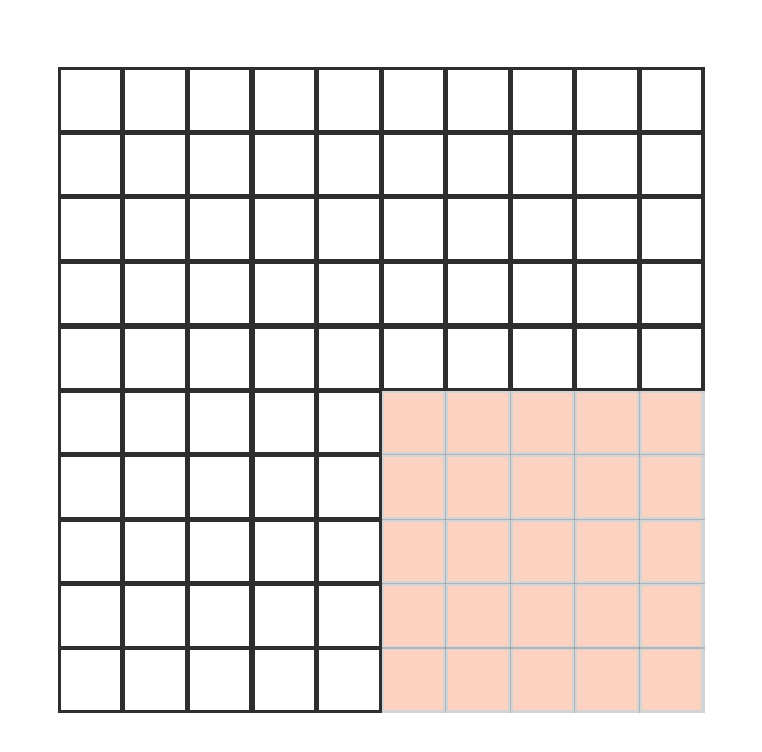
\includegraphics[scale=.25]{pictures/Kuva13-2-75.pdf}
        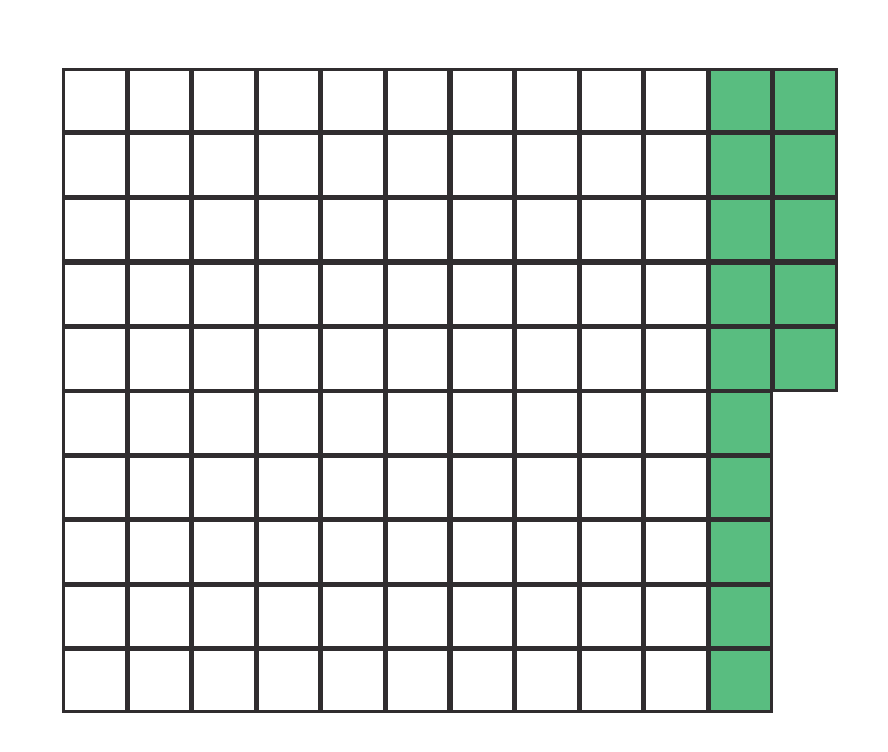
\includegraphics[scale=.25]{pictures/Kuva13-3-115.pdf}
    \end{center}
\end{esimerkki}

% MUUTOSPROSENTTI
\laatikko{
Prosentteja käytetään usein ilmaisemaan suureiden muutoksia, esimerkiksi luku $a$ kasvaa luvuksi $b$. \termi{muutosprosentti}{Muutosprosenttia} laskettaessa muutoksen suuruutta verrataan alkuperäiseen lukuun. Perusarvona on siis alkuperäinen arvo, johon nähden muutos on tapahtunut. Muutosta merkitään yleensä symbolilla $\Delta$ (kreikan kielen suuri \textit{delta}).
    
    \termi{absoluuttinen muutos}{Absoluuttinen muutos} luvusta $a$ lukuun $b$ on $b-a$.
    \termi{suhteellinen muutos}{Suhteellinen muutos} saadaan suhteuttamalla absoluuttinen muutos alkuperäiseen lukuun $a$ eli laskemalla
 \[ \Delta_{\text{suhteellinen}} = \frac{\Delta_{\text{absoluuttinen}}}{a} = \frac{b-a}{a} \]
    
Muutosprosentti saadaan suhteellisesta muutoksesta muuttamalla se prosenttiluvuksi
\[ \Delta_{\text{prosentti}} = \Delta_{\text{suhteellinen}} = \frac{b-a}{a} \] tulkittuna prosenteissa.

} %liikaa laatikkoa

\begin{esimerkki}
Vesan paino on tammikuussa $68$\,kg ja kesäkuussa $64$\,kg.
    \alakohdat{
§Mikä on Vesan painon \textit{absoluuttinen muutos}?
§Mikä on Vesan painon \textit{muutosprosentti}?
}
    
	\begin{esimratk}
	\alakohdat{
§Halutaan tietää Vesan painon \textit{absoluuttinen muutos} eli muutos kiloina tammikuusta kesäkuuhun.
    \[
       \Delta_{\text{absoluuttinen}} = b - a = 64\,\text{kg} - 68\,\text{kg} = -4\,\text{kg}
    \]

Vesan paino on muuttunut $-4$ kiloa, eli Vesa on laihtunut 4 kiloa.

§Halutaan tietää Vesan painon muutos \textit{prosentteina} tammikuusta kesäkuuhun.
    
    \[\Delta_{\text{prosentti}}
        = \frac{\Delta_{\text{absoluuttinen}}}{a}
        = \frac{-4}{68}
        \approx -0,06
        = -6\,\%   \]
    
Vesan paino on muuttunut kuudella prosentilla negatiiviseen suuntaan, eli Vesa on laihtunut kuusi prosenttia.
   } 
    \end{esimratk}
    \begin{esimvast}
    \alakohdat{
§Vesa on laihtunut $4$ kiloa.
§Vesa on laihtunut $6\,\%$.
 }
    \end{esimvast}
\end{esimerkki}

% EROTUSPROSENTTI
\laatikko{
    Muutosprosentille läheinen käsite on \termi{erotusprosentti}{erotusprosentti}. Erotusprosentti ilmaisee kuinka monta prosenttia jokin on suurempi tai pienempi kuin joku toinen. Suhteellinen erotus saadaan laskemalla lukujen absoluuttinen erotus $|b-a|$ ja vertaamalla sitä perusarvoon, joka on aina ``kuin''-sanan jälkeinen arvo.
    
Jos luku $a$ on $p\,\%$ pienempi tai suurempi kuin luku $b$, pätee
    \[ p = \frac{|b-a|}{b}. \]
}
    
\begin{esimerkki}
Miniluumutomaatit maksavat normaalisti $4,80$ euroa kilolta. Nyt ne ovat kuitenkin alennuksessa ja maksavat $2,50$ euroa kilolta.
     \alakohdat{
     §Kuinka monta prosenttia enemmän miniluumutomaatit maksavat normaalisti kuin alennuksessa?
     § Kuinka monta prosenttia vähemmän miniluumutomaatit maksavat alennuksessa kuin normaalisti?
    } 
	\begin{esimratk}
     
     \alakohdat{
 §Verrataan absoluuttista erotusta alennettuihin miniluumutomaatteihin:
\begin{align*}
     &\frac{|b-a|}{b}  = \frac{|2,50-4,80|}{2,50} = \frac{|-2,30|}{2,50} \\
     = &\frac{2,30}{2,50}  = 0,92 = 92,0\,\%.
\end{align*}
§Verrataan absoluuttista erotusta normaalihintaisiin miniluumutomaatteihin:
\begin{align*}
     &\frac{|b-a|}{a} = \frac{|2,50-4,80|}{4,80} = \frac{|-2,30|}{4,80} \\
     = &\frac{2,30}{4,80}  \approx 0,479  = 47,9\,\%.
\end{align*}
	 }
\end{esimratk}
		
     \begin{esimvast}
      \alakohdat{
     §Miniluumutomaatit maksavat normaalisti $92,0$\,\% enemmän kuin alennuksessa.
     §Miniluumutomaatit maksavat alennuksessa $47,9$\,\% vähemmän kuin normaalisti.
     }
     
Huomataan, että se mihin verrataan, on merkittävää.
      \end{esimvast}
     \end{esimerkki}

Joissain tilanteissa perusarvo on tuntematon. Se ratkeaa usein kätevästi yhtälöllä.
% MUUTOSKERTOIMESTA PIENI TEORIAPLÄJÄYS?
\begin{esimerkki}
Tuotteen hintaa korotettiin $15$\,\%, jolloin hinnaksi muodostui $175$\,euroa. Kuinka suuri oli alkuperäinen korottamaton hinta?
	\begin{esimratk}
Olkoon alkuperäinen hinta $x$\,euroa. Koska hintaa on korotettu $15$\,\%, on uusi hinta $115$\,\% alkuperäisestä eli alkuperäinen hinta $x$ on kerrottu $1,15$:llä:
\begin{align*}
	1,15x	&= 175	&	&|\, \text{Jaetaan} 1,15\text{:llä}.\\
	x	&= \frac{175}{1,15} \approx 152,17
\end{align*}
	\end{esimratk}
    \begin{esimvast}
    Tuotteen alkuperäinen hinta oli $152,17$\,euroa.
    \end{esimvast}
\end{esimerkki}

Huomaa, että edellisessä esimerkissä saatuun kertoimeen $1,15 = 115\,\%$ oltaisiin päädytty myös laskemalla $x + 0,15x = (1 + 0,15)x = 1,15x$.

Lauseella ''kaksi kertaa enemmän'' tarkoitetaan usein yleiskielessä kaksinkertaista. Matemaattisesti nämä ovat kuitenkin eri asioita. Sekaannuksen vuoksi on syytä olla käyttämättä tällaista ilmaisua.

% PROSENTTIYKSIKKÖ
\laatikko{
\termi{prosenttiyksikkö}{Prosenttiyksikköä} käytetään mittaamaan prosenttilukujen absoluuttista muutosta. Esimerkiksi $3\,\%$ on yhden prosenttiyksikön suurempi kuin $2\,\%$, mutta $50\,\%$ suurempi kuin $2\,\%$. Jos prosenttiluku muuttuu, muutos voidaan ilmaista joko prosentteina (suhteellinen muutos) tai prosenttiyksikköinä (absoluuttinen muutos).
}

Prosentin ja prosenttiyksikön merkitysero on keskeinen esimerkiksi talousuutisten tulkinnassa.

\begin{esimerkki}
    Tuotteen markkinaosuus on vuoden tammikuussa $10$\,\% ja kesäkuussa $15$\,\%.
    \alakohdat{
    §Kuinka monta prosenttia tuotteen markkinaosuus on noussut tammikuusta kesäkuuhun?
    §Kuinka monta prosenttiyksikköä tuotteen markkinaosuus on noussut tammikuusta kesäkuuhun?
    }

    \begin{esimratk}
    \alakohdat{
    §Tuotteen markkinaosuuden muutos prosentteina:
          \[
                \frac{15-10}{10} = \frac{5}{10} = 0,5 = 50\,\%.
          \]
	§Tuotteen markkinaosuuden muutos prosenttiyksiköinä $15\,\%-10\,\%=5\,\%$
	}
    \end{esimratk}

\begin{esimvast}
\alakohdat{
§$50$ prosenttia
§$5$ prosenttiyksikköä
}
\end{esimvast}
\end{esimerkki}
